%%%%%%%%%%%%%%%%%%%%%%%%%%%%%%%%%%%%%%%%%
% Simple Sectioned Essay Template
% LaTeX Template
%
% This template has been downloaded from:
% http://www.latextemplates.com
%
% Note:
% The \lipsum[#] commands throughout this template generate dummy text
% to fill the template out. These commands should all be removed when 
% writing essay content.
%
%%%%%%%%%%%%%%%%%%%%%%%%%%%%%%%%%%%%%%%%%

%----------------------------------------------------------------------------------------
%	PACKAGES AND OTHER DOCUMENT CONFIGURATIONS
%----------------------------------------------------------------------------------------

\documentclass[12pt]{article} % Default font size is 12pt, it can be changed here

\usepackage{geometry} % Required to change the page size to A4
\geometry{a4paper} % Set the page size to be A4 as opposed to the default US Letter

\usepackage{graphicx} % Required for including pictures

\usepackage{float} % Allows putting an [H] in \begin{figure} to specify the exact location of the figure
\usepackage{wrapfig} % Allows in-line images such as the example fish picture

\usepackage{lipsum} % Used for inserting dummy 'Lorem ipsum' text into the template

\linespread{1.2} % Line spacing

%\setlength\parindent{0pt} % Uncomment to remove all indentation from paragraphs

\graphicspath{{Pictures/}} % Specifies the directory where pictures are stored

\usepackage{listings}

\begin{document}

%----------------------------------------------------------------------------------------
%	TITLE PAGE
%----------------------------------------------------------------------------------------

\begin{titlepage}

\newcommand{\HRule}{\rule{\linewidth}{0.5mm}} % Defines a new command for the horizontal lines, change thickness here

\center % Center everything on the page

\textsc{\LARGE Tsinghua Univerisity}\\[1.5cm] % Name of your university/college
\textsc{\Large Computational Biology}\\[0.5cm] % Major heading such as course name
\textsc{\large Lecture 9: April 21, 2014}\\[0.5cm] % Minor heading such as course title

\HRule \\[0.4cm]
{ \huge \bfseries Sequence Assembly}\\[0.4cm] % Title of your document
\HRule \\[1.5cm]

\begin{minipage}{0.4\textwidth}
\begin{flushleft} \large
\emph{Scribe:}\\
Weiyi \textsc{Chen} % Your name
\end{flushleft}
\end{minipage}
~
\begin{minipage}{0.4\textwidth}
\begin{flushright} \large
\emph{Lecturer:} \\
Dr. Michael \textsc{Zeng} % Supervisor's Name
\end{flushright}
\end{minipage}\\[4cm]

{\large \today}\\[3cm] % Date, change the \today to a set date if you want to be precise

%\includegraphics{Logo}\\[1cm] % Include a department/university logo - this will require the graphicx package

\vfill % Fill the rest of the page with whitespace

\end{titlepage}

%----------------------------------------------------------------------------------------
%	TABLE OF CONTENTS
%----------------------------------------------------------------------------------------

\tableofcontents % Include a table of contents

\newpage % Begins the essay on a new page instead of on the same page as the table of contents 

%----------------------------------------------------------------------------------------
%	INTRODUCTION
%----------------------------------------------------------------------------------------

\section{Introduction} % Major section
In bioinformatics, sequence assembly refers to aligning and merging fragments of a much longer DNA sequence in order to reconstruct the original sequence. This is needed as DNA sequencing technology cannot read whole genomes in one go, but rather reads small pieces of between 20 and 30000 bases, depending on the technology used. Typically the short fragments, called reads, result from shotgun sequencing genomic DNA, or gene transcript (ESTs). [Myers, E. W., 2000]

%------------------------------------------------

\subsection{The Sequencing Problem} % Sub-section
Sequencing machines cannot read the entire genomic sequence, but can read fragments. As stated, DNA sequencing technology cannot read whole genomes in one go, but rather reads small pieces of between 20 and 30000 bases, depending on the technology used. Therefore we need to make use of dividing and conquering approach. 
\begin{itemize}
\item Shear whole DNA sequence into millions of small fragments
\item Read ~500 - 700 nucleotides each time from small fragments 
\item Assemble the sequenced fragments
\end{itemize}

%------------------------------------------------

\subsection{Different Sequencing Methods} % Sub-section
The complexity of sequence assembly is driven by two major factors: the number of fragments and their lengths. While more and longer fragments allow better identification of sequence overlaps, they also pose problems as the underlying algorithms show quadratic or even exponential complexity behavior to both number of fragments and their length. And while shorter sequences are faster to align, they also complicate the layout phase of an assembly as shorter reads are more difficult to use with repeats or near identical repeats. [Batzoglou, S., 2002]

%------------------------------------------------

\subsubsection{Sanger sequencing: 800bp-1000 bp}
In 1975, the Sanger sequencing was invented and until shortly after 2000, the technology was improved up to a point where fully automated machines could churn out sequences in a highly paralleled mode 24 hours a day. Large genome centers around the world housed complete farms of these sequencing machines, which in turn led to the necessity of assemblers to be optimized for sequences from whole-genome shotgun sequencing projects where the reads are about 800-900 bases long.

\subsubsection{454 sequencing: 300-400 bp}
By 2004 / 2005, pyrosequencing had been brought to commercial viability by 454 Life Sciences. This new sequencing method generated reads much shorter than those of Sanger sequencing: initially about 100 bases, now 400-500 bases. Its much higher throughput and lower cost (compared to Sanger sequencing) pushed the adoption of this technology by genome centers, which in turn pushed development of sequence assemblers that could efficiently handle the read sets. [Google group]

\subsubsection{Illumina Genome Analyzer: 35-150 bp}
From 2006, the Illumina (previously Solexa) technology has been available and can generate about 100 million reads per run on a single sequencing machine. Compare this to the 35 million reads of the human genome project which needed several years to be produced on hundreds of sequencing machines. Illumina was initially limited to a length of only 36 bases, making it less suitable for de novo assembly (such as de novo transcriptome assembly), but newer iterations of the technology achieve read lengths above 100 bases from both ends of a 3-400bp clone.

\subsubsection{Helicos: 30bp}
Announced at the end of 2007, the Helicos assembler by Dohm et al. was the first published assembler that was used for an assembly with Solexa reads. It was quickly followed by a number of others. [Dohm, J. C.; 2007]

%----------------------------------------------------------------------------------------
%	MAJOR SECTION 1
%----------------------------------------------------------------------------------------

\section{Sequence Assembly Algorithms} % Major section

The problem of sequence assembly can be compared to taking many copies of a book, passing each of them through a shredder with a different cutter, and piecing the text of the book back together just by looking at the shredded pieces. [Myers, E. W., 2000]

%------------------------------------------------

\subsection{Shortest Superstring Problem (SSP)} % Sub-section
The problem is defined as finding a shortest fragment that contains all of the reads, given a set of strings. Specifically,
\begin{itemize}
	\item Parameter: $(s_1, s_2, ..., s_n)$ as strings
	\item Return: a fragment $s$, such that contains all strings $(s_1, s_2, ..., s_n)$ as substrings and the length of $s$ is minimized
\end{itemize}

%------------------------------------------------

\subsubsection{Assumptions} % Sub-sub-section

There are some assumptions of the problem,
\begin{itemize}
	\item We do not consider errors with parameters, which states all reads are 100\% accurate
	\item No repeats: we do not consider identical reads in different genome region, which is to say identical reads must be from the same genome region
	\item Given demands, the optimized return or solution is defined as the shortest string.
\end{itemize}

%------------------------------------------------

\subsubsection{Example} % Sub-sub-section

\begin{itemize}
	\item Parameter: \{ACG, CGA, CGC, CGT, GAC, GCG, GTA, TCG\}
	\item Return: TCGACGCGTA (length 10)
\end{itemize}
This is an NP-hard problem. Note that sequencing errors are ignored here.

%------------------------------------------------

\subsection{Reducing SSP to Traveling Salesman Problem (TSP)} % Sub-section
The traveling salesman problem (TSP) asks the following question: Given a list of cities and the distances between each pair of cities, what is the shortest possible route that visits each city exactly once and returns to the origin city? It is an NP-hard problem in combinatorial optimization, important in operations research and theoretical computer science. Since this is a problem we have already analyzed, we can reduce SSP to the 
maximum Traveling salesman problem (TSP), and then analyze TSP.

%------------------------------------------------

\subsubsection{Implementation of Reduction} % Sub-sub-section
\begin{itemize}
\item Define overlap $(s_i, s_j)$ as the length of the longest prefix of $s_j$ that matches a suffix of $s_i$.
\item Make graph with $n$ vertices representing $n$ reads $s_1,�s_2, ...,�s_n$.
\item Insert negative edges of length overlap $(s_i, s_j)$ between vertices $s_i$ and $s_j$.
\item Find the shortest path which visits every vertex exactly once.
\end{itemize}

%------------------------------------------------

\subsubsection{Example}
Suppose the parameters are $S=\{ATC, CCA, CAG, TCC, AGT\}$, then SSP will be like \\
\centerline{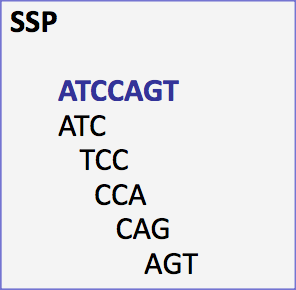
\includegraphics[scale=0.5]{note1}}
And TSP will be like \\
\centerline{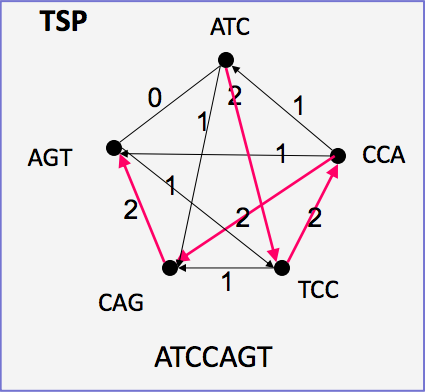
\includegraphics[scale=0.5]{note2}}
Unfortunately we have millions of reads and the TSP is NP-complete. What can we do? It's "Eulerian Path". We will talk about that later.

%------------------------------------------------

\subsection{Greedy Algorithm} % Sub-section
Given a set of sequence fragments the object is to find the shortest common super-sequence. The greedy algorithm to solve TSP is
\begin{enumerate}
\item calculate pairwise alignments of all fragments
\item choose two fragments with the largest overlap
\item merge chosen fragments
\item repeat step 2. and 3. until only one fragment is left
\end{enumerate}
The result is a suboptimal solution to the problem. The conjecture says that the Greedy Algorithm has approximation factor 2 for the shortest superstring problem. Currently the best bound of the approximation factor for the greedy algorithm is 3.5. It's still an open problem.

\subsubsection{Example}

An example is shown in graph below, where the assembler joins, in order,  reads 1 and 2 (overlap = 200 bp), then reads 3 and 4 (overlap  = 150 bp), then reads 2 and 3 (overlap = 50 bp) thereby creating a single contig from the four reads provided in the input.  One disadvantage of the simple greedy approach is that because local information is considered at each step, the assembler can be easily confused by complex repeats, leading to mis-assemblies. \\
\centerline{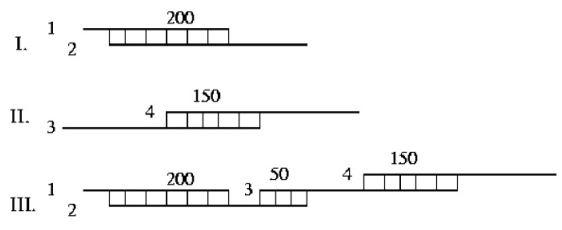
\includegraphics[scale=0.5]{greedy}}

%------------------------------------------------

\subsection{Overlap Layout Consensus} % Sub-section
The relationships between the reads provided to an assembler can be represented as a graph, where the nodes represent each of the reads and an edge connects two nodes if the corresponding reads overlap.  

\subsubsection{Overlap Graph}
A graph (G) consists of vertices (V) and edges (E)
$$ G = (V, E) $$
Edges can either be directed (directed graphs) or undirected (undirected graphs). The order of a graph is $|V|$ (the number of vertices). A graph's size is $|E|$, the number of edges. The degree of a vertex is the number of edges that connect to it, where an edge that connects to the vertex at both ends (a loop) is counted twice.

Overlap graph: For a set of sequence reads S, construct a directed weighted complete graph 
$$G = (V,E,w)$$
where one vertex per read in the graph, and 
$$w(v_i,v_j) = overlap(s_i,s_j)$$
$overlap()$ is the length of longest suffix of $s_i$ that is a prefix of $s_j$.

\subsubsection{Example}
The assembly problem thus becomes the problem of identifying a path through the graph that contains all the nodes - a Hamiltonian path in the below graph. This formulation allows to use techniques developed in the field of graph theory in order to solve the assembly problem.  An assembler following this paradigm starts with an overlap stage during which all overlaps between the reads are computed and the graph structure is computed.  In a layout stage, the graph is simplified by removing redundant information.  Graph algorithms are then used to determine a layout (relative placement) of the reads along the genome.  In a final consensus stage, the assembler builds an alignment of all the reads covering the genome and infers, as a consensus of the aligned reads, the original sequence of the genome being assembled.

\centerline{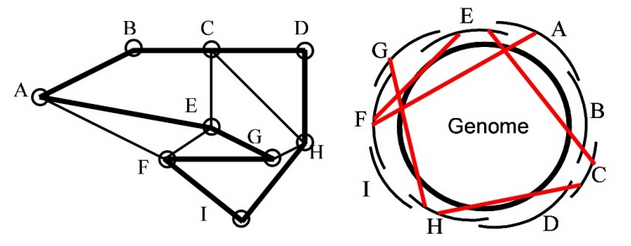
\includegraphics[scale=0.5]{olc}}

The thick edges in the picture on the left (a Hamiltonian cycle) correspond to the correct layout of the reads along the genome (figure on the right).  The remaining edges represent false overlaps induced by repeats (exemplified by the red lines in the figure on the right).

Unfortunately similar to the Traveling salesman problem, finding Hamiltonian path is an NP-complete problem, Checking whether a graph has a Hamiltonian path or not is very difficult.

%------------------------------------------------

\subsection{Eulerian path} % Sub-section
In graph theory, an Eulerian trail (or Eulerian path) is a trail in a graph which visits every edge exactly once. Similarly, an Eulerian circuit or Eulerian cycle is an Eulerian trail which starts and ends on the same vertex. They were first discussed by Leonhard Euler while solving the famous Seven Bridges of K�nigsberg problem in 1736. Mathematically the problem can be stated like this:

Given the graph below, is it possible to construct a path (or a cycle, i.e. a path starting and ending on the same vertex) which visits each edge exactly once?

\centerline{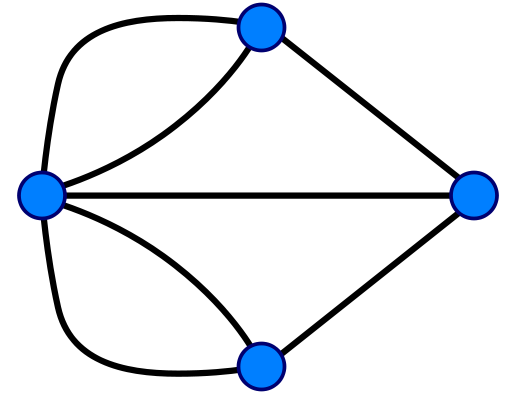
\includegraphics[scale=0.3]{Konigsburg_graph}}

\subsubsection{Properties}
\begin{itemize}
\item An undirected graph has an Eulerian cycle if and only if every vertex has even degree, and all of its vertices with nonzero degree belong to a single connected component.
\item An undirected graph can be decomposed into edge-disjoint cycles if and only if all of its vertices have even degree. So, a graph has an Eulerian cycle if and only if it can be decomposed into edge-disjoint cycles and its nonzero-degree vertices belong to a single connected component.
\item An undirected graph has an Eulerian trail if and only if at most two vertices have odd degree, and if all of its vertices with nonzero degree belong to a single connected component.
\item A directed graph has an Eulerian cycle if and only if every vertex has equal in degree and out degree, and all of its vertices with nonzero degree belong to a single strongly connected component. Equivalently, a directed graph has an Eulerian cycle if and only if it can be decomposed into edge-disjoint directed cycles and all of its vertices with nonzero degree belong to a single strongly connected component.
\item A directed graph has an Eulerian trail if and only if at most one vertex has (out-degree) - (in-degree) = 1, at most one vertex has (in-degree) - (out-degree) = 1, every other vertex has equal in-degree and out-degree, and all of its vertices with nonzero degree belong to a single connected component of the underlying undirected graph.
\end{itemize}

\subsubsection{Eulerian Cycle Algorithm}
\begin{itemize}
\item Start at any vertex v, traverse unused edges until returning to v
\item While the cycle is not Eulerian: 
\begin{itemize}
\item pick a vertex w along the cycle for which there are untraversed outgoing edges
\item traverse unused edges until ending up back at w
\item join two cycles into one cycle
\end{itemize}
\end{itemize}

\subsubsection{Assembly algorithms}
Eulerian path approaches are based on early attempts to sequence genomes through a technique called sequencing by hybridization.  In this technique, instead of generating a set of reads, scientists identified all strings of length k (k-mers) contained in the original genome. While this experimental method did not produce a viable alternative to Sanger sequencing, it led to the development of an elegant approach to sequence assembly. This approach, also based on a graph-theoretic model, breaks up each read into a collection of overlapping k-mers.  Each k-mer is represented in a graph as an edge connecting two nodes corresponding to its k-1 bp prefix and suffix respectively.  It is easy to see that, in the graph containing the information obtain from all the reads, a solution to the assembly problem corresponds to a path in the graph that uses all the edges - an Eulerian path.  One advantage of the Eulerian approach is that repeats are immediately recognizable while in an overlap graph they are more difficult to identify.

According to the statement above, we can construct a deBruijn graph: 
\begin{itemize}
\item Edges represent $k$-mers that occur in $s$
\item Vertices correspond to $(k-1)$-mers
\item Directionality goes from the $k-1$ prefix to the $k-1$ suffix \\
\centerline{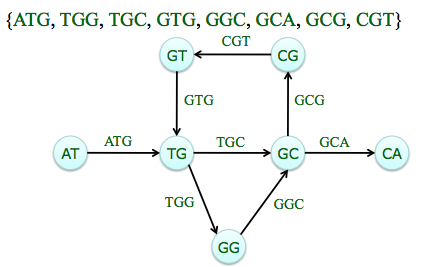
\includegraphics[scale=0.5]{eulerian}}
\item Find a DNA sequence containing all k-mers, which corresponds to find a path that visits every edge of the graph exactly once.
\end{itemize}

%----------------------------------------------------------------------------------------
%	CONCLUSION
%----------------------------------------------------------------------------------------

\section{Conclusion} % Major section

Assembly is a Complicated Problem. Besides the obvious difficulty of this task, there are some extra practical issues: the original may have many repeated paragraphs, and some shreds may be modified during shredding to have typos. Excerpts from another book may also be added in, and some shreds may be completely unrecognizable. 

For the repeats, it is hard to know where repeats begin or end, whether reads are not long enough, possibility that human genome has many different repeats and gene duplications. For the sequencing errors, it is hard to distinguish true from error-based overlaps too.

%----------------------------------------------------------------------------------------
%	BIBLIOGRAPHY
%----------------------------------------------------------------------------------------

\begin{thebibliography}{99} % Bibliography - this is intentionally simple in this template

\bibitem[Myers, E. W., 2000]{Myers, E. W.: 2000}
Myers, E. W.; Sutton, GG; Delcher, AL; Dew, IM; Fasulo, DP; Flanigan, MJ; Kravitz, SA; Mobarry, CM et al. (March 2000).
\newblock A whole-genome assembly of Drosophila
\newblock {\em Science}, 287 (5461): 2196-204.
 
 \bibitem[Batzoglou, S., 2002]{Batzoglou, S.: 2002}
Batzoglou, S.; Jaffe, DB; Stanley, K; Butler, J; Gnerre, S; Mauceli, E; Berger, B; Mesirov, JP; Lander, ES (January 2002).
\newblock ARACHNE: a whole-genome shotgun assembler
\newblock {\em Genome Research}, 12 (1): 177-89.

\bibitem[Google group]{Google group}
Copy in Google groups
\newblock post announcing MIRA 2.9.8 hybrid version
\newblock {\em Usenet group}

 \bibitem[Dohm, J. C., 2007]{Dohm, J. C.: 2007}
Dohm, J. C.; Lottaz, C.; Borodina, T.; Himmelbauer, H. (November 2007).
\newblock SHARCGS, a fast and highly accurate short-read assembly algorithm for de novo genomic sequencing
\newblock {\em Genome Research}, 17 (11): 1697?706.

\end{thebibliography}

%----------------------------------------------------------------------------------------

\end{document}